% @TODO Change this
\chapter{Introduction}
\label{chapter1}

* ----- <roadsign> Peter Construction Co. </roadsign> *

% @TODO Do metheorologoy as an example
Modern science relies heavily on data collection and analysis. The only way to test a scientific hypothesis in practise is to conduct an experiment that is in accordance to the theory and to collect data outputted by the experiment. Through analysing the collected data scientists can reason about the probability of whether their hypothesis is correct. If that probability is not high enough the hypothesis is rejected and a better one is sought. The analytical current machinery for doing so is reliable and robust. It is based on statistics, machine learning and *other stuff*. One major issue is that more data can be collected than can be analysed []. The only solution to this problem is to reduce the amount of data. The central problem with this approach is in picking which pieces of data to discard. Ideally one would like to discard data which is of little significance and would slow down the analysis with little to offer in terms of important insight and information.

This is where computational topology can come in. Topology is about the qualitative features of spaces. These are the big scale general features that are essential in making a space what it is. Computational Topology is concerned with extracting those from data. This is why it is useful in our case.

An invaluable tool in learning about data is visualisation. In fact the same problem hold with scientific and information visualisation. The human eyesight has limited capabilities. Ensuring only relevant and important information is displayed is crucial in the success of such methods. Let us take for example a tool such as the contour tree. It is primarily used as a discrete summary of the connectivity of a scalar field.

*Show example and explain it.*

Through the contour tree we can accomplish the following amazing things. Give examples.

The first aim of this dissertation will to be aid in the speeding up of the construction of the contour tree from raw data. In the modern world where individual cores of processors are not expected to become much faster practical speedup has to come from leveraging parallelism be it distributed or shared memory. 

The second aim of this dissertation is to discuss the simplification of contour trees and how that can be approached from two different perspectives in the realm of computational topology. 

%Statistics can play a huge role in deciding. There are well enstablished methods for discarding correlated predictors

Computational Topology 



What is computational topology?
What are the primary tools that are used?
Where have they been used in practise and with what success.

Talk about why performance can be lacking.
Talk about parallel algorithms.
Talk about the future of computation.

Outline what you will do in the thesis.
Go though the contents in the chapters.


The mathematics covered in this dissertation are far too broad to be presented in all their magnificence. This is why rather than attempting to introduce the theory in the classical textbook fashion of definition-theorem-proof I have opted out for focusing more on developing intuition behind the big ideas at play. I do so because I will later rely on the reader's intuition in presenting examples and the further technical developments of the subject of computational topology in the recent years. 

\section{Set Theoretic Notation}


\begin{defn} Let $X$, $Y$ be two sets and $f$ be a function between them. Let $A \subseteq Y$ the preimage of $A$ under $f$ is defined as the points in $X$ which are mapped onto $A$. It is denoted as $f^{-1}(A) = \{x \in X : f(x) \in A\}$  \end{defn}

Note that taking the preimage of a set does not require $f$ to be invertable.

\section{Point Set Topology}

Topology is the mathematical field that studies continuous change between topological spaces. Any set $X$ can be a topological space as long as we defined a collection of subsets of $X$ called open sets. The open sets represent elements of $X$ which are "near" or "close" to one another. If we have two topological spaces $X$ an $Y$ and wish to study how one can be continuously mapped to the other we instead focus on how the open sets are mapped. The open sets provide certain structure on the sets and we would like to study the functions that preserve that structure and focus on the properties of spaces that are invariant under such functions. Those functions are what we call the continuous functions.

Let us now be more formal now and define these notions precisely.

\begin{defn} Let $X$ be a set and $\tau$ be a set of subsets of $X$. The set $\tau$ is a topology on $X$ when the following holds:  \end{defn}

\begin{itemize}
    \item $X \text{ and } \emptyset \in \tau$.
    \item If $U \text{ and } V \in \tau$ then $U \cap V \in \tau$.
    \item If $\{U_\lambda\}_{\lambda \in \Lambda}$ is a family of subsets of $X$, where $U_\lambda \in \tau$ for all $\lambda \in \Lambda$, then 
        $\bigcup_{\lambda \in \Lambda}{U_\lambda} \in \tau$.
\end{itemize}

\begin{defn} Let $(X, \tau)$ be a topological space. Any subset of $A \subseteq X$ which is in $\tau$ is said ot be open.  \end{defn}

\begin{defn} Let $(X, \tau)$ be a topological space. Let $x \in X$ be any element of $X$. We will call $x$ a point in $X$ and we will call any open set $A$ containing $x$ an open neighbourhood of $x$.  \end{defn}

%@TODO Redo this setence
The pair $(X, \tau)$ is called a topological space. In practice one builds a topology by first figuring out how they would like their open sets to look like and then takes all unions and finite intersections to obtain the full topology.

\begin{ex} The standard topologly on $\mathbb{R}$.  \end{ex}

The standard topology on $\mathbb{R}$ is build from subsets of $\mathbb{R}$ called open balls. The open ball centered at $x \in \mathbb{R}$ with radius $\epsilon \in \mathbb{R}^+$ is a subset $B_\epsilon(x)$ of $\mathbb{R}$ defined as:

$$ B_\epsilon(x) = \{y \in \mathbb{R} : |x - y| < \epsilon \} .$$

These are all the points whose distance from $x$ is less than $\epsilon$. The collection of all open balls as $x$ ranges over $\mathbb{R}$ and $\epsilon$ ranges over $\mathbb{R}^+$ makes up the building blocks of the topology. The open sets in the topology are all the open balls together with their arbitrary unions and finite intersections.


\begin{ex} The standard topologly on $\mathbb{R}^n$.  \end{ex}

We can slightly adjust the previous definition to obtain a topology on $\mathbb{R}^n$. We just have to consider $\vec{x} \text{ and } \vec{y}$ to be vectors in $\mathbb{R}^n$ and evaluate the distance between them using the standard Eucledian metric. That is if $\vec{x} = (x_1, ..., x_n)$ and $\vec{y} = (y_1, ..., y_n)$ then:

$$ B_\epsilon(\vec{x}) = \{\vec{y} \in \mathbb{R}^n : \sqrt{\sum_{i = 1}^{n}{(x_i - y_i) ^ 2}} < \epsilon \} $$

is a subset of $\mathbb{R}^n$ with all points of distance less than $\epsilon$ from $\vec{x}$. Like previously the topology on $\mathbb{R}^n$ is obtained through arbitrary unions and finite intersections of the set of open balls.


One may notice that the topology we put on a set is by no means unique. If we wish we may even use the topology made up of \em all \em subsets of a given set. That topology is not preferred because introduces very little structure to our topological space. As we will shortly see it makes the question of continuity rather moot. Topologist prefer topologies that introduce structure on a space that is both intuitive and reflective of the properties they wish to study. The standard metric is useful because Eucledian distance is the natural quantifier of how "near" things are in almost all applied mathematical models. While the information about the actual distance is lost in the generality of the topology, the structure it imposes allows us to talk about important global properties of spaces such as path-connectednes and compactness.

Having a topology on $\mathbb{R}^n$ is all well and good but in this dissertation we shall work with surfaces and triangulations of surfaces in $\mathbb{R}^2$ and $\mathbb{R}^3$. If we had to define a topology on them in a similar fashion we would not get far. Luckily subsets of topological spaces can naturally inherit the topology of their superset.

\begin{defn} Let $(X, \tau_X)$ be a topological space and $A$ be a subset of $X$. The subspace topology of $A$ is defined as: \end{defn}

$$ \tau_A = \{U \cap A: U \in \tau_X\}.$$

To obtain all open sets of $A$ take the open sets in $X$ and remove from them all points which are not in $A$. Going further we will consider any surface embedded in $\mathbb{R}^2$ and $\mathbb{R}^3$ to have the subspace topology of the standard topology unless otherwise stated.

We are finally ready to present the definition of a continuous function. 

\begin{defn} A function $f : X \to Y$ is said to be continuous when the preimage of an open set in $Y$ is an open set in $X$. \end{defn}

In formal notation if $U \in Y$ is open in $Y$ then $f^{-1}(U)$ is open in $X$. This definition captures the intuitive understanding we have of continuity - if we "slightly adjust" the output of a function in $Y$ then there should be only a "slight change" in input in $X$. The "slight change" is formalised by considering all points in a single open set, as we can think of them as being "near". This is the reason why continuous functions are colloquially described as manipulating an object in space without glueing together parts of it or making holes in it. Those disrupt the open sets.

So far we have obtained the means of endowing any subset of $\mathbb{R}^n$ with a topology and we have outlined a general recipe for creating continuous function between them - have open sets be the preimage of open sets. We will now introduce our first topological invariant. But first we shall show how we can "move" around in a topological space. 

%@TODO Maybe introduce connectedness
\begin{defn} Let $X$ be a topological space and let $x, y \in X$ be any two points. A path between $x$ and $y$ in $X$ is a continuous function $f: [0, 1] \to X$ such that $f(0) = x$ and $f(1) = y$.  \end{defn}

    This is analogous to the definition of a close curve from differential geometry. The main difference being that we have no notion of differentiability or smoothness yet. As an example think of the space $X$ as a surface in $\mathbb{R}^3$ and two distinct points $x$ and $y$ on it. A path between $x$ and $y$ is a curve that starts at $x$, moves around the surface and ends at $y$.

\begin{defn} A topological space $X$ is said to be path-connected if there exists a path between any two points $x, y \in X$  \end{defn}


This deceptively simple looking definition actually holds the overarching methodology for reasoning about algebraic invariants of topological spaces. In this case we have employed a two parameter family of utility functions to "measure" a global property of the topological space. The two parameter family is the collection of all paths between all pairs of points.

\begin{prop} The continuous image of a path-connected space is path-connected. \end{prop}

    Notice that in this definition we have implied surjectivity. Indeed if $X, Y$ are topological spaces such that $X$ is path-connected and $Y$ is not and $f : X \to Y$ is a continuous function then all we can say is that $im(f)$ is path-connected.

Lastly we must explore how topological spaces are viewed by topologist. After all if two spaces share all of their topological properties should they be considered different? See coffee mug and dognut example []. We shall make this precise with the notions homeomorphism and homotopy equivalence.

\begin{defn} Two topological spaces $X$ and $Y$ are said to be homeomorphic when there exists a bijetion $f : X \to Y$, such that $f$ and $f^{-1}$ are continuous. Furthermore the function $f$ is called a homeomorphism between $X$ and $Y$.  \end{defn}

Homeomorphism is the appropriate equivalence relation for topological spaces. For example if we have two homeomorphic topological spaces $X$ and $Y$ and we know one of them has a particular topological property, then the other one will have it as well. Conversely if we know that a space is path connected and another one isn't, then they are not homeomorphic.

In the realm of algebraic topology there is another equivalence relation that is more flexible than this and still preserve the algebraic invariants of spaces. Before presenting it we must first introduce homotopy of functions.


\begin{defn} Let $X$ and $Y$ be two topological spaces. Let $f, g: X \to Y$ be two continuous functions. We say that $f$ and $g$ are homotopic when there exists a third continuous function $H:X \times [0, 1] \to Y$ such that:  \end{defn}

\begin{itemize}
    \item $H(x, 0) = f(x), \forall x\in X$
    \item $H(x, 1) = g(x), \forall x\in X$
\end{itemize}

We can think of homotopy as a one parameter family of functions $\{f_t\}_{t \in [0, 1]}$ such that $f_0 = f$ and $f_1 = g$. Homotopy defines an equivalence relation on all continuous functions between $X$ and $Y$. This notion can be extended to topological spaces as follows:


\begin{defn} Two topological spaces $X$ and $Y$ are said to be homotopy equivalent if there exist two continuous functions $f: X \to Y$ and $g: Y \to X$ such that:  \end{defn}
\begin{itemize}
    \item $f \circ g$ is homotopic to $i_X$ 
    \item $g \circ f$ is homotopic to $i_Y$,
\end{itemize}

where $i_X$ and $i_Y$ are the identity functions on $X$ and $Y$ respectively.

Intuitively we can think of homotopy as a continuous deformation of the image of one of the functions to the image of the other. One can readily observe that every homeomorphism is a homotopy equivalence. Let $g = f^{-1}$, then $f \circ g = i_X$ and $g \circ f = i_Y$ as $f$ is a bijection and every function is homotopic to itself. However the converse is not true and a homotopy equivalence is not a homeomorphism.

In a way very similar to abstract algebra continuous function play the role of homomorphisms and homeomorphisms play the role of isomorphisms. Also note that homotopy equivalence does not necessarily preserve all topological properties of a topological space. They do however preserse those which we care about such as path-connected and algebraic structures defined on the topological spaces. We will prefer to use them instead of homeomorphisms. 


\begin{defn}{Topological Invairant}   \end{defn}

*I will add more things to this chapter later if I need to*


% @TODO Redo this chapter!
\section{Building Blocks}

The most basic building blocks in Computational Algebraic Topology are Abstract Simplical Complexes (ASC) and Simplicial Complexes (SC). Abstract Simplical Complexes are a combinatorial structure aimed at generalising discrete graphs. Simplicial Complexes are their geometric realisation in standard Eucledian Space. For example a planar graph $G = (V, E)$ is an ASC as a collection of vertices (singleton sets) and edges (sets of two elements). An embedding in the plane with points representing vertices and line segments (or curves) between them as edges is a Simplicial Complex.

*Show Example*

Let us introduce these concepts more formally starting with ASC and then demonstrating how they can be realised in Euledian Space via SC.

\begin{defn} Given a set $V$, an Abstract Siplicial Complex called $\Delta$ on $V$ is a collection of subsets of $V$ such that if $\sigma \in \Delta$ and $\varphi \subseteq \sigma$ then $\varphi \in \Delta$.  \end{defn}

In the spirit of keeping our definitions computationally tractable we will only consider ACS of finite sets. Elements of $\Delta$ are called simplices. The dimension of a simplex is it's cardinality minus one. To connect this to geometry simplices of dimension zero are called vertices and simplices of dimension one are called edges. To generalise further two dimensional simplices are called triangles and three dimensional simplices are called tetrahedra. Simplices of higher dimension lose their geometric flavour, so will avoid naming them altogether.

 %We will denote by $\Delta_n \subseteq \Delta$ all simplices in $\Delta$ of dimension $n$.

\begin{ex} Show a simple example of an abstract simplical complex. \end{ex}


% @TODO This is main not accurate
\begin{defn} Let $\sigma$ be an n-simplex in $\Delta$. A face of $\sigma$ is any simplex $\varphi$ in $\Delta$ such that $\varphi \subseteq \sigma$. \end{defn}

We will call the faces of a simplex that have $k$ dimensions less it's codimension $k$ faces. The codimension one of a tetrahedra are the triangles. The codimension two faces are the edges and so on. 

An ASC is closed under taking subsets, so the faces of a simplex are in fact all subsets of the simplex. This is also one of the reasons why high dimensional ASC are avoided in practise. For example an n-dimensional simplex has $2^n$ faces which are all in the complex by definition.

\begin{defn} Let $V$ be a finite set and $\Delta$ an ASC of $V$. Let $\sigma \in \Delta$. The star of $\sigma$ is the set of all simplices of which $\sigma$ is a face. In set theoretic notation:\end{defn}

$$ St(\sigma) =  \{ \varphi \in \Delta : \sigma \subset \varphi \}. $$


* REDO THIS OR LEAVE IT OUT*
% @TODO Redo This or leave it out.
The interplay between continuous mathematics and combinatorics is indeed interesting. For example in this context the star of a vertex plays the role of an open neighbourhood. We can define a topology on an ASC called the Alexandroff topology.

% @TODO Find a reference for this.

\begin{defn} The collection of all start in an ASC $\Delta$ is basis for a topology. The topology is finitely generated by $\{St(\sigma)\}_{\sigma \in \Delta}$.  \end{defn}



% @TODO Explain why/where this is useful.

While ASC are a purely combinatorial construct, we saw in our example in the beginning of the section that like graphs they do have a geometric realisation. We will now provide the definitions of how their geometric realisation can be constructed via simplicial compexes.

% Comb Topo Book
\begin{defn} The standard geometric n-simplex is the convex hull of the set of endpoints of the standard basis $[1, 0, ..., 0], [0, 1, ..., 0], ..., [0, 0, ..., 1]$ in $\mathbb{R}^{n+1}$ defined as: \end{defn}


% From Hatcher
$$ \Delta^n = \{(t_0, t_1, ..., t_n) \in \mathbb{R}^{n+1} : \sum_{i = 0}^{n} t_i  = 1 \text{ and } t_i \ge 0, \forall i = 0, 1, ..., n \} $$

We will define the face of an n-simplex analogously as:

\begin{defn} A face of the standard geometric n-simplex is the convex hull of a subset of endpoints of the standard basis $[1, 0, ..., 0], [0, 1, ..., 0], ..., [0, 0, ..., 1]$ in $\mathbb{R}^{n+1}$ defined as: \end{defn}

\begin{ex} Show an example of the basic simplices. \end{ex}

A Simplical Complex $K$ is the finite collection of homeomorphic images of standard simplicies such that:

\begin{itemize}
    \item If the simplex $\sigma$ is in $K$ then all of it's faces must also be in $K$.
    \item The intersection of the images of two simplicies is either empty or a common face of both.
\end{itemize}

You can imagine using the standard simplicies as building blocks for a Simplical Complex. We take them, embed them in a high enough dimensional Eucledian space and glue them together along their common faces. Self intersections are of course not allowed. In fact every ASC has a geometric realisation, but not necessarily in their original dimension. This is made precise by the following theorem \cite{comp-topo}.

\begin{thm} Every abstract simplicial complex of dimension $n$ has a geometric realization in $\mathbb{R}^{2d+1}$. \end{thm}



% @TODO Analogous to Hatcher
%In order to build a fully functional simplical complex we extend by definitions by the following. The union of all faces of $\Delta^n$ is the boundary of $\Delta^n$ and it is written as $\partial \Delta^n$. The open simplex $\overset{\circ}{\Delta^n}$ is just $\Delta^n \textbackslash \partial \Delta^n$ as is the interior of $\Delta^n$.


% @TODO From Herbert
%We can now define a simplical complex $\Delta$ embedded in $\mathbb{R}^n$ as the finite collection of homeomorphic images of simplices of dimension no more than $n$. Furthermore if $\sigma \in \Delta$ then all of the faces $\varphi \subset \sigma$ must be in $\Delta$, and $\sigma_1, \sigma_2 \ in \Delta$ implies that their intersection $\sigma_1 \cap \sigma_2$ is either empty of a face of both.



% @TODO From Hatcher (modified)

%A simplical complex structure of a topological space $X$ with vertex set $V$ and ASC $\Delta$ defined on $V$ is a collection of homeomorphic maps $\{f_\sigma : \Delta^{|\sigma|} \to X\}_{\sigma \in \Delta}$ such that:


%\begin{itemize}
    %\item If $f_\sigma$ is one of the maps and $\varphi \subset \sigma$ then the image of $f_\varphi$ is a subset of the image of $f_\sigma$.
    %\item If $f_\sigma$ is one of the maps no other map maps to the image of the restriction $f_\sigma | \overset{\circ}{\Delta^{|\sigma|}}$.
    %\item If $f_{\sigma_1}$ and $f_{\sigma_2}$ are such maps then then the intersection of their images $im(f_{\sigma_1}) \cap im(f_{\sigma_2})$ is the image $im(f_\varphi)$ where $\varphi$ is a face of both. 

%\end{itemize}


%% @TODO Herbert


%\begin{thm} Geometric Realisation Theorem. Every abstract simplicial complex of dimension $d$ has a geometric realisation in $\mathbb{R}^{2d+1}.$   \end{thm}



\section{Vector Spaces, Quiver Diagrams and Barcode Diagrams}

*This chapter will probably be redistributed in the homology chapter. I'll probably remove it.*

Should I define a vector space, bases, etc.?

Should I define a vector space, bases, etc.?


%Suppose we have a number of vector spaces with linear maps between con
Suppose we have a number of vector spaces $(V_1, V_2, ...,V_n)$

Suppose we have a number of vector spaces $(V_1, V_2, ...,V_n)$ together with linear maps $(f_1, f_2, ...,f_{n-1})$ that that map between consecutive vector spaces like follows : $f_i: V_i \to V_{i+1}, \forall i = 1, 2, ..., n -1$. 

A quiver representation is a directed multigraph where the vertices are sets and directed edges are function between sets. In our case the vertices will be vector spaces and the edges linear maps. The quiver diagram of the configuration we just described looks as follows:

$$V_1 \overset{f_1}{\longrightarrow} V_2 \overset{f_2}{\longrightarrow} ... \overset{f_{n-1}}{\longrightarrow} V_n  $$


"This sounds weird, fix it."
Not that we can always extend any sequence of vector spaces with the null vector space and the null maps as follows:

$$ 0 \longrightarrow ... \longrightarrow 0 \longrightarrow V_1 \overset{f_1}{\longrightarrow} V_2 \overset{f_2}{\longrightarrow} ... \overset{f_{n-1}}{\longrightarrow} V_n  \longrightarrow 0 \longrightarrow ... \longrightarrow 0$$

A barcode diagram is a digram that shows which shows how the basis elements of the vector spaces evolve as they get mapped through the linear functions once we commit to particular basis elements for each vector space.

Show a barcode diagram.

A Chain Complex is a quiver representation where the image of each maps is a subset of the kernel of the next one.

$$ ... \longrightarrow V_1 \overset{d_1}{\longrightarrow} V_2 \overset{d_2}{\longrightarrow} ... \overset{d_{n-1}}{\longrightarrow} V_n  \longrightarrow ... $$

This example is a chain complex when $im(d_k) \subseteq ker(d_{k+1})$. As the image is a subset of the kernel the we can equivalently write this as the composition $d_{k+1}d_k = 0$. In practical terms once we commit to baseis multiplying consecutive matricies will equal the zero matrix. An important property of the barcode diagram of chain complexes is that no line can be longer than two units!


\begin{ex}  A Simple Chain Complex \end{ex}
Let us now for simplicity and demonstrational purposes assume that each $V_i$ is isomorphic to $\mathbb{R}^n$ for some $n \in \mathbb{Z}$.


% @TODO Continue this.
An exact sequence is a chain complex where $im(d_k) = ker(d_{k+1})$. Exact sequences are useful because of the nice properties like ...

The homology of a chain complex is defined as a quantifier of how far a chain complex is from being an exact sequence. It is defined as: $ H_k = ker(d_{k+1}) / im(d_k) $

Let $V$ be a vector space and $W$ a subspace of $V$. A coset of $W$ is the set $v + W = \{v + w : w \in W\}$.

A quotient in a vector space is defined in the following way: 

$$ V/W = \{v + W: v \in V\} = \{\{v + w : w \in W\} : v \in V \}$$

Show a picture of the cosets.

Luckily in $\mathbb{R}^n$ we have the following theorem: $\mathbb{R}^n / \mathbb{R}^m \simeq \mathbb{R}^{n - m} $ where we have slightly abused notation as $\mathbb{R}^m$ can not be a subspace of $\mathbb{R}^n$, but we consider it isomorhpic to one for $m \le n$.

$$ \mathbb{R}^3 {\longrightarrow} \mathbb{R}^2 {\longrightarrow} \mathbb{R}^4 $$


\section{Algebraic Topology}


% @TODO Define a topological invariant.
% @TODO Make sure you have the definition of n-cycle

Algebraic Topology concerns itself with topological invariants of algebraic nature. These invariants are obtained through the extraction of algebraic structures like groups, rings, vector spaces or modules from a topological space. One of the leading formalisms in algebraic topology is Homology. Homology measures properties of a topological space such as connected components, number of holes (1-cyles), number of voids (2-cycles) or more generally number of n-cycles with the use of vector spaces. Before introducing the mathematical apparatus by which homology is built we will take a short detour to explore the concepts that lead to it's inception.

%Continuous images of topological spaces preserve the structure of these algebraic objects in the sense they they can be used to produced homomorphism between them. 

\subsection{Euler Characteristic}

The first topological invariant of algebraic nature we shall encounter is the Euler Characteristic. It is denoted as $\chi$ and it assigns an integer to suitably nice spaces through a generalisation of counting \cite{elementary-applied-topology}. The concept was originally defined for polyhedra as a alternating sum of the form $|V| - |E| + |F|$, where $V$ is the set of vertices, $E$ the set of edges and $F$ the set of faces. This allowed for the classification of the Platonic solids [fig].


% @TODO Define CW complexes, simplical complexes may not generalise polyhedra
The Euler Characteristic can be generalized to all spaces that can be decomposed into a finite number of cells. Let us first consider simplical complexes because they generalise polyhedra. The natural generalisation of the alternating sum is to continue it indefinitely with the number of 3-cells, then 4-cells, etc., as follows

$$ \chi = k_0 - k_1 + k_2 - ... = \sum_{i}{(-1)^i~k_i}, $$

where all $k_i$ is the number of $i$ dimensional simplicies and $k_i = 0$ for $i$ bigger than some $n \in \mathbb{Z}^+$ and all $k_i$ for $i \le n$ are positive integers. 


Even more generally given a topological space $X$ that can be decomposed into the disjoint union of a finite number of open cells $X = \coprod_{\alpha}\sigma_{\alpha}$ where each k-cell $\sigma_{\alpha}$ is homeomorphic to $\mathbb{R}^k$ we can apply the same formula as above \cite{elementary-applied-topology}. 

$$ \chi(X) = \sum_{\sigma}{(-1)^{dim(\sigma)}} .$$

\begin{lem}   The Euler Characteristic is homotopy invariant. \end{lem}

This results allows to compute in practice $\chi$ of manifolds by considering any of their finite triangulations. As long as there is a homeomorphism between a manifold and triangulation $\chi$ will not change. We will be well advised to pick the triangulations with the least number of simplices to improve computational efficiency. For example the octahedron is a triangulation of a sphere and therefore the Euler Characteristic of the sphere is zero. For further information on this subject we refer the reader to [].

\subsection{Homology}

The guiding principle behind the Euler Characteristic was to decompose a space into cells, count them and perform cancellations based on the parity of the dimension of the cells. This approach yields important information about a topological space, but we can hope to gain more by generalising it. We shall accomplish this by leveraging the mathematical machinery of Homology. Homology is a tool that was first developed to measure the topological complexity high dimensional manifolds \cite{persistence-original} by identifying what other manifolds can be embedded or surround them. For example with homology we can detect that there is a hole in the torus.

The theory of Homology comes in two flavours - \textbf{simplical} and \textbf{singular}. Simplicial homology is geared towards analysing simplical complexes and singular homology is the appropriate generalisation for arbitrary topological spaces. In this dissertation we restrict attention on singular homology because we are primarily interested in the computational aspect of homology. For this weed tractable spaces. We will however on occasion refer to singular homology when we desire to leverage a more general result from the relevant theory. More information on singular homology can be found in the following sources \cite{algebraic-topology, elementary-applied-topology}


% @TODO Finish this
Homology is built around the interplay between the two key concepts of \textbf{cycles} and \textbf{boundaries}. Let us consider the simplical complex depicted on Figure \ref{fig:hom-sc} as an example. It consists of four vertices $\{a, b, c, d\}$, five edges $\{ab, bc, ca, db, cb\}$ and one face $\{abc\}$. The boundary of a simplex consists of its codimension-1 faces. For example the boundary of the 1-dim simplex $ab$ consists of the 0-dim simplices $a \text{ and } b$. The boundary of the 2-dim simplex $abc$ consists of the 1-dim simplices $ab, ac \text{ and } cb$. A cycle on the other hand consists of the simplices that form the boundary of a simplex that is of one dimension higher (regardless of whether that bigger simplex is in the complex). In our example we can observe that the edges $ab, bc, ca$ and $bd, dc, cb$ form a 1-dim cycle.  This also happens to be in line with the graph theoretic definition. The first and last vertex of the paths formed by those edges are the same. A more geometric way to put it is that the edges enclose an 2-dim area of space.  To expand this definition to higher dimensional cycles picture the faces of the tetrahedron. They would form a 2-cycle as they completely enclose a 3-dim volume. In general an n-cycle consists of simplices that are the boundary of a n+1-dim simplex

\begin{figure}[h]%
    \centering
    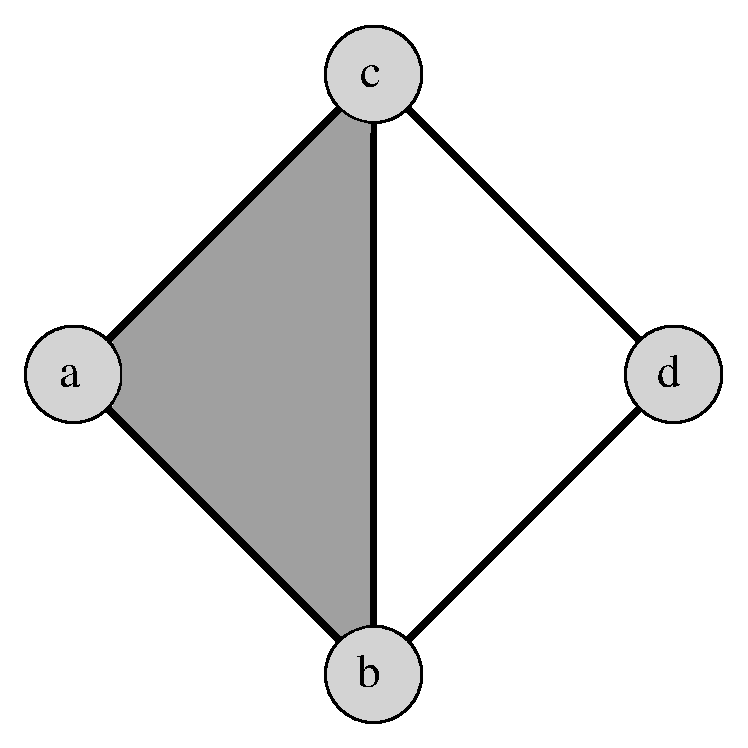
\includegraphics[scale=0.4]{./images/chapter1/homology-sc.eps}%
    \caption{An Example Simplical Complex}%
    \label{fig:hom-sc}%
\end{figure}




Notice also that the paths formed by the edges $bc, ca, ab$ and $ca, ab, bc$ are also cycles. The only difference is which vertex they start and end at. We would like to disregard the choice of starting point completely because those three paths represent the same structure in the simplical complex. To this end we shall introduce additive algebraic notation. In this notation the same cycle would be written as $ab + bc + ca$.  We will soon demonstrate that additive notation is not only used to illustrate the point of disregarding edge order. Its more important aspect is that it allows us to treat sums of edges as linear combinations in an abstract vector space.

The interplay between between cycles and boundaries is in asking the question - which cycles in the complex are \textbf{not} the boundary of a higher dimensional simplex. This is important because these cycles cannot be contracted to a point. The lack of higher dimensional simplex the enclose means there is a void of some dimension in our simplex.

Let us be more formal now. To begin with, we will operate with vector spaces over the field of coefficients $\mathbb{Z}_2 = \{0, 1\}$ together with the standard operations of addition and multiplication modulo two. We could develop the same theory with the familiar coefficient in $\mathbb{R}$ but we would sacrifice geometric intuition and computational efficiency later on. The building blocks of the homology of a simplical complex $X$ are:


\begin{itemize}
    \item The \textbf{vector spaces of n-chains} of $X$. This is denoted as $C_n(X)$. It is an abstract vector space with basis all the n-simplices of $X$ for $n \in \{0, 1, 2, ..., \}$.
    \item The \textbf{boundary maps} of the n-chains of $X$. These are linear maps between consecutive vector spaces of n-chains. It is denoted as $\partial_n : C_n(X) \to C_{n-1}(X)$.
\end{itemize}

In our previous example $C_0(X)$ was the vector space that is spanned by the vertices $\{a, b, c, d\}$. We write this as $C_0(X) = span(\{a, b, c, d\})$. A vector in $C_0(X)$ is a linear combination of the basis vectors using coefficients in $\mathbb{Z}_2$. Let $\sigma \in C_0(X)$ be a vector, then we can express it as $\sigma  = \alpha_0a + \alpha_1b + \alpha_2c + \alpha_3d$ where $\alpha_i \in \{0 ,1\}$ for every $i = 0, 1, 2, 3$. Going a dimension up $C_1(X) = span(\{ab, bc, ca, cd, bd\})$. As we pointed out earlier the cycle that consists of the edges $bc, cd, db$ is represented by the sum or linear combination $bc + dc + bd = 0ab + 1bc + 0ca + 1cd + 1bd$ and has coordinates $(0, 1, 0, 1, 1)$ in $C_1(X)$ with respect to the basis we have chosen.

* Badly explained redo this *
We may of course wish to work with to use a different basis for some of the n-chains. The operation of change of basis is useful in linear algebra and can have an effect on the computational efficiency, especially when dealing with projections and quotient spaces. We can use any linear combinations of the simplicies so long as they have the same span and form a basis. For example $C_0(X) = span(\{a + b, b, c, c + d\})$ because the vectors $(1, 1, 0, 0), (0, 1, 0, 0), (0, 0, 1, 0) \text { and } (0, 0, 1, 1,)$ are linearly independent.

The boundary maps are defined analogously to how we presented them in the beginning of the section. The effect a boundary map has on a basis element $\sigma \in C_n(X)$ is that it returns the linear combination consisting of basis elements of $C_{n-1}(X)$ that are codimension-1 faces of $\sigma$. If $\sigma$ is the affine combination of the vertices $[v_0, v_1, ..., v_n]$ then we define it's boundary as:

$$ \partial(\sigma) = \partial([v_0, v_1, ..., v_n]) = \sum_{i=0}^{n}[v_0, ... , \hat{v_i}, ..., v_n] $$

We would also like to extend $\partial$ linearly. Linear functions commute with vector addition and scalar multiplication. This allows us to know everything that is to know about a linear function through it's effect on the basis vectors of its domain. This is because in the general setting for a linear function $f : V \to W$ we have that: $ f\big(\sum_{i}{a_iv_i}\big) = \sum_i{a_if(v_i)} $. We have demonstrated the effects of $\partial_n$ on the basis vectors of $C_n(X)$. All we have to do is extend it linearly. This results in the following definition:


$$ \partial\bigg(\sum_{\sigma}a_{\sigma}\sigma\bigg) = \partial\bigg(\sum_{\sigma}{a_{\sigma}[v_{\sigma_0}, v_{\sigma_1}, ..., v_{\sigma_n}]}\bigg) = \sum_{\sigma}{a_{\sigma} \sum_{i=0}^{n}[v_{\sigma_0},..., \hat{v}_{\sigma_i}, ..., v_{\sigma_n}]} .$$


% @TODO Chain complex more generally.
What we have thus obtained is a collection of vector spaces together with linear maps between. We will call it a chain complex. This is the quiver representation of a chain complex of a simplicat comples of dimension n.


$$ C_n(X) \overset{\partial_n}{\longrightarrow} C_{n-1}(X) \overset{\partial_{n-1}}{\longrightarrow} ... \overset{\partial_2}{\longrightarrow} C_1(X) \overset{\partial_1}{\longrightarrow} C_0(X) $$

For convenience we can extend this chain on both sided with the zero dimensional vector space as follows:

$$ 0 \overset{\partial_{n+1}}{\longrightarrow} C_n(X) \overset{\partial_{n}}{\longrightarrow} C_{n-1}(X) \overset{\partial_{n-1}}{\longrightarrow} ... \longrightarrow C_1(X) \overset{\partial_1}{\longrightarrow} C_0(X) \overset{\partial_0}{\longrightarrow} 0. $$

In this sequence $\partial_{n+1} \text{ and } \partial_{0}$ are zero maps. In the case of $\partial_{n+1}$ it maps the zero vector of $0$ to the zero vector of $C_n(X)$ and $\partial_0$ maps all vectors in $C_0(X)$ to the zero vector in $0$.

Let us now translate the geometric intuition we have of cycles and boundaries to domain of algebra. The boundaries are provided to us by the boundary maps. Thus the set of all boundaries in $C_n(X)$ is given by the image of $C_{n+1}(X)$ under $\partial_{n+1}$ or $im(\partial_{n+1})$. The cycles in $C_n(X)$ are given by all the vectors in $C_n(X)$ that go to the zero vector of $C_{n-1}(X)$ under $\partial_n$. Intuitively the boundary of an n-chain is zero exactly when all of the faces of the simplices in the chain have even parity and cancel in our binary algebra. The set of all vectors that go to the zero vector under the boundary map $\partial$ is precisely the kernel of $\partial$ or $ker(\partial)$.

From linear algebra we know that for a linear function $f: V \to W$, $ker(f)$ is a linear subspace of $V$ and $im(f)$ is a subspace of $W$. In the context of chain complexes this means that the images and kernels of all the boudary maps are linear subspaces of their respective n-chains. Before learning how the interplay between cycles and boundaries is translated in this setting we must present the following fundamental theorem

\begin{lem} Fundamental Lemma of Homology. $(\partial_{n-1} \circ \partial_n) (\sigma) = 0, \text{ for every } \sigma \in C_{n}(X)$. \end{lem}

\begin{proof}
    We will only sketch the intuitive outline of the proof and refer the reader to \cite{algebraic-topology} for a more complete version.

    Let us consider the boundary of $\sigma \in C_n(X)$ which is $\partial_n(\sigma)$. It contains all of the n-1 faces of $\sigma$. Furthermore every n-2 face of $\sigma$ belongs to exactly two n-1 faces of sigma. Therefore they will cancel out in the second boundary operation $\partial_{n-1}\partial_n(\sigma)$.
\end{proof}


\begin{cor}  For every two consecutive boundary maps $\partial_n$ and $\partial_{n-1}$ in a chain complex $im(\partial_n) \subseteq ker(\partial_{n-1})$. \end{cor}

\begin{proof}
    If the image of $\partial_n$ were not in the kernel of $\partial_{n-1}$ then there would be at least one n-chain $\sigma$ for which $(\partial_{n-1} \circ \partial_n) (\sigma) \ne 0$. By the Fundamental Lemma of Homology this is not possible.
\end{proof}


% @TODO and example
* Add the definitions of quotient in the appendix *

We can obtain the kernel as a way of detecting the cycles in chain complex. But how can we disregard the cycles that are covered by a boundary? The answer is another algebraic operation. The quotient of the cycles and their subspace the boundaries. What the quotient operation does is to effectively send all cycles that consist entirely of boundaries to zero. *Show example with previous example*. This is precicely how we define the n-th homology of a chain map.


\begin{defn} The n-th homology group of a chain map is vector space $H_n(X) = ker(\partial_{n+1})\big/im(\partial_n)$. \end{defn}

From linear algebra \cite{lin-alg-done-right} we know two important things about the quotient $H_n(X)$. The first one is that the quotient of a vector space and its subspace is a vector space. The second one is that the dimension of the quotient space is equal to the difference of the dimension of the vector space and the dimension of the subspace. Therefore $H_n(X)$ is a vector space and $dim(H_n(X)) = dim(ker(\partial_{n+1})) - dim(im(\partial_n))$. Elements of the homology groups are called homology classes.

*I will now give you some example of homology computations. Connect them to Euler characteristic*

% @TODO Redo this
Now that we have ventured into the algebra and computed something based on the topology of the space it is time to interpret those results. 
What we are most interested is the dimension of the homology groups. The dimension of a finite dimensional vector space is the number of vectors in a basis of that vector space. Thus if $H_n(X) \simeq \mathbb{Z}_2^m$ then $dim(H_n(X)) = m$. The dimensions of the homology groups are also known as the Betti numbers. The Betti numbers have the following topological interpretation.


\begin{itemize}
    \item Betti zero - $b_0$ is the number of connected components
    \item Betti one - $b_1$ is the number one dimentional holes in a space or holes.
    \item Betti two - $b_3$ is the number two dimentional holes in a space or voids.
\end{itemize}


% @TODO What is nice enough?
The higher order Betti numbers represent the number of higher dimensional holes. Given a nice enough topological space we can expect the Betting numbers from a point onwards to all be zero. This of course means that the according homology group are the zero dimensional vector space.

*Give example with the torus*

This is exactly what we wanted from Homology. An apparatus that allows us distinguish topological spaces based on the connectivity of their n-dimensional simplical complexes.

* Leave this or not? *

Before going forward we must note that we did not have to use coeficients in $\mathbb{Z}_2$ we could have equally used coeficients in $\mathbb{Z}$ but $\mathbb{Z}$ is not a field and we would have obtained that the $C_n(X)$ and $H_n(X)$ are not vector spaces but free abelian groups. If instead we had picked any arbitrary ring we would have obtained free modules instead of free abelian groups. We did indeed lose some information but sticking to vector spaces. The Betti numbers are not always equal, but by the Coeficient Theorem they are for suitably nice spaces. We readily refer the reader to \cite{algebraic-topology} to learn about those. We shall continue the treatment of the subject in the same spirit of vector spaces.


There are two more notions we need to define to be able to fully utilise the power of homology - that of reduced and relative homology.

The need for reduced homology arises from a slight inconsistency in the interpretation of the homology groups. Take for example the topological space that consists of a single point. In that topological space all homology groups except for the $H_0$ are trivial. It is convenient in many application to make $H_0$ behave like the rest of the homology group and specifically be trivial in our example. In this sense path-connected topological spaces will have trivial zeroth homology. The geometrical interpretation of this extension is the reduces 0th homology counts the number of voids that separate path connected components of a topological space.

In formal terms we augment the chain complex of a topological space $X$ with one additional group $\mathbb{Z}$.

$$ ... \longrightarrow C_1(X) \longrightarrow C_0(X) \overset{\epsilon}{\longrightarrow} \mathbb{Z}_2 \longrightarrow 0 $$

In this augmented chain the function $\epsilon: C_0(X) \to \mathbb{Z}_2$ is defined as $\epsilon\big(\sum_{i}n_i\sigma_i\big) = \sum_{i}n_i$. The value of $\epsilon$ is equal to the parity of the number of simplicies in the chain. We will define the reduces homology as the homology of the augmented chain complex or $\overset{\sim}{H}_n(X)$. We have that $\overset{\sim}{H}_n(X) = H_n(X)$ for $n > 0$ and $\overset{\sim}{H}_0(X) \bigoplus \mathbb{Z}_2 = H_0(X) $

Another useful notion is that of relative homology. Just as in abstract algebra we can extract useful properties of quotient groups a natural question to ask is whether we can do something similar in the setting of algebraic topology and quotient spaces. 

Let $A$ be a subcomplex of $X$. Let us then define $C_n(X, A) = C_n(X) / C_n(A)$ and define a new relative chain complex as

$$ ... \longrightarrow C_n(X, A) \longrightarrow ... \longrightarrow C_1(X, A) \longrightarrow C_0(X, A) \longrightarrow 0. $$

This is a chain complex because...

% @TODO Explain Why
More importantly the relative homology $H_n(X, A)$ is not defined as $H_n(X) / H_n(A)$ but as the homology of the chain complex defined above. As the boundary maps take $C_n(A)$ to $C_{n-1}(A)$ the boundary maps induce relative boundary maps on the chain complex. We call the cycles and boundaries of the relative chain complex relative chains and relative boundaries.

Intuitively here is how we can think of the relative homology classes \cite{algebraic-topology}.

A relative chain $\alpha$ is a relative cycle when it's boundary $\partial\alpha $ is in $C_n(A)$.

A relative cycle $\alpha$ is trivial in the homology when it's the sum of a boundary $\partial \beta$ of $\beta \in C_{n+1}(X)$ and a chain $\gamma \in C_n(A)$.

There is a way to relate the this purely algebraic machinery to our geometric intuition for "nice" enough spaces.


% @TODO Give example with disc and sphere!


% @TODO Finish this.
\begin{thm} Excision - Let $X$ be a topological space, let $A \subseteq X$ and let $U \subseteq A$ where the closure of $U$ is contained in the interiour of $A$. Then   \end{thm}


A corollary of this is that if $A$ is a close subcomplex of $X$ then $H_n(X, A) \simeq \overset{\sim}{H}_n(X/A, A/A)$ where $A/A$ is a single point in $X/A$. This allows us to leverage our geometric intuition about quotient space to compute homology groups.



\section{Differential Topology}

Differential topology is the study of differentiable function on differentiable manifolds. As opposed to the theory of differential geometry, topologists are predominantly interested in the global structure of manifolds and primarily disregard local information such as for example curvature because it can be of little value in investigating the global properties of a space such as its genus. The classical example that illustrates this is that of the doughnut and the coffee mug. From the point of view of differential geometry they are not the same. You cannot rotate and translate one of them to obtain in other. From the differential topology perspective they are indistinguishable in that they share all the global properties topology can "see".   

\subsection{Morse Theory}

One of the leading fields of differential topology is that of Morse Theory. It has shown to be fruitful in both theoretical investigations and real world application and computation []. Morse theory is the study of the deep relation between spaces and function defined on them. One of the main goals is to determine the shape of a shape by analysing a functions that can be defined on it. 

Consider for example the real line $\mathbb{R}$ and the circle $S^1$. There are differentiable functions from $\mathbb{R}$ to $\mathbb{R}$ such as $y = x$ which do not take a minimum or a maximum value. They can be arbitrary large or small on the manifold $\mathbb{R}$. It is not possible to define such a differentiable function from $S^1$ to $\mathbb{R}$. This is due to the maximum value theorem. More formally a differentiable function is continuous and $S^1$ is compact. By [] the continuous image of a compact space is compact and by [] the compact spaces of $\mathbb{R}$ are closed and bounded. Closed and bounded means unions of intervals of the form $[a, b]$ where $|a|, |b| < \epsilon$ for some $\epsilon \in \mathbb{R}$. We can pick the lower bound of the interval with the lowest lower bound and the upper bound of the interval with the highest upper bound for the minimum and maximum values. Therefore any differentiable function defined on $S^1$ will take a minimum and a maximum value.

This example demonstrates the general methodology of Morse Theory. One defines a function on a smooth manifold and studies the manifold through the function. A more concrete to do is by using the critical points of that function as means of learning about the "shape" of the manifold. The class if real valued function on a manifold is far too complex though. This is why Morse Theory restricts it's attention to Morse functions.


\begin{defn} A function $f: M \to \mathbb{R}^n$ is a Morse Function if $f$ is smooth and at critical points the Hessian (matrix of second partial derivatives) is full rank.   \end{defn}

Based on this definition we will defined level sets, sublevel sets and superlever sets of a Morse function.

\begin{defn} A level set at a value $h$ of a Morse function $f: M \to \mathbb{R}$ is the set $f^{-1}(\{h\}) = \{x \in M: f(x) = h \}$   \end{defn}

Sublevel sets are defined in terms of intervals of the interval $[-\infty, a]$ and are the preimage $f^{-1}([-\infty, a]) = \{x \in M: f(x) \in [-\infty, a] \}$. Superlevel sets are defined analogously in terms of intervals of the form $[a, -\infty]$. We shall call the path-connected components of a level set contours.

These sub(super) level sets allows us to decompose the manifold and work with chunks of it at a time.

Morse functions ensures the following properties which we will make use of in the future:

\begin{itemize}
    \item None of the critical points are degenerate.
    \item In Morse functions topological changes of the sub(super)level sets only happen at critical values. 
    \item A Morse function defined on a close surface has a finite number of critical points.
\end{itemize}

\subsection{Reeb Graph}


% @TODO Define the quotient topology.


The Reeb Graph is a tool that encapsulates the evolution of the level sets of a continuous function. It does so by tracking how the connected connected components in the level sets appear, disappear and split or join together. When the function is Morse, an edge in the Reeb Graph corresponds to a sequence of connected components in the level sets whose topology does not change. The vertices correspond to critical points where the topology of those components does changes (when they appear, dissapear, split or join). Morse theory ensures that critical points occur at distinct values of the parameter and are isolated. This removes any ambiguities that may arise in the construction of the graph. Furthermore that fact that their number is finite on a close surface and the fact that they only happen at critical values make this computation tractable.


\begin{defn}
Given a topological space $X$ and a continuous function $f: X \to \mathbb{R}$ we can define an equivalence relation $\sim$ such that two points $x, y$ in $X$ are equivalent when there exists a path between them in a level set $f^{-1}(\{h\})$ for some $h \in \mathbb{R}$. The Reeb Graph is the quotient space $X \big/ \sim$ together with the quotient topology.
\end{defn}

Intuitively it contracts all connected components to a single point.

*SHOW LOTS OF PICTURES*


% @TODO Define a topological graph.
The Reeb Graph is indeed homeomorphic to a topological graph. *Explain Why*

There are two important equations that \cite{comp-topo} relate the Betti Numbers of the topological space $X$ and the quotient space $X \big/ _\sim$

$$ \beta_0(X \big/ _\sim) = \beta_0(X) $$
$$ \beta_1(X \big/ _\sim) \le \beta_1(X) $$.

We remind the reader that a contractable domain is on that is homotopic to single point. In the homology of such a space there is only one connected component and all other homology groups are trivial. Therefore $\beta_0 = 1 \text{ and } \beta_n = 0, n \in {1, 2, ...}$. A direct consequence of this is that the Reeb Graph of a contractable space is a tree regardless of the function defined on it.

\subsection{Contour Tree}

The special case of the Reeb Graph of a contractable space is called a Contour Tree. 

*Write about the algorithm for computing reeb graphs, say why they are slow*

In order to move forward with the state of the art algorithms for computing the contour tree due to Carr, et. at []. We will define an additional equivalence relation on the quotient space that relates contour of different level sets.


\begin{defn}  Let $C = \{p_0, p_1, ..., p_n\}$ be the set of all critical points where the number of connected components in the level sets changes. \end{defn}

* Not sure if this definition works *

\begin{defn}   
    Let $\alpha_1, \alpha_2$ be be two contours of two level sets (possibly the same level set). Then $\alpha_1 \sim \alpha_2$ when there exists a homotopy between $\alpha_1$ and $\alpha_2$ that does not pass through any point in $C$ or when $\alpha_1 = \alpha_2$.
\end{defn}


% @TODO What about those contours?
Intuitively if we can deform one of the contours to the other along $X$ without passing through a saddle then both contours correspond to the same edge in the contour tree. How about the contours that pass through critical points? They are only equivalent to themself because any homotopy to any other contour must pass through at least one critical point - the one contained in the contour.


\begin{defn} We will call contour classes with an infinite number of members infinite contour classes. Those correspond to the edges of the contour tree.  \end{defn}

\begin{defn} We will call contour classes with a single members finite contour classes. Those correspond to the vertices of the contour tree.  \end{defn}

Finite contour classes also correspond to closed sets of the form $[a, a] = \{a\}$ where $a$ is the value of a critical point.

Infinite contour classes correspond to open sets of the form $(a, b)$ where $a \text{ and } b$ are the values of critical points and where for any two $c, c' \in (a, b)$ there is a contour in $f^{-1}(\{c\})$ that is equivalent to a contour in $f^{-1}(\{c'\})$.

Leafs correspond to local minima or maxima.

Interior vertices are one where at least one infinite contour class is created and at least one infinite class is destroyed \cite{hamish-masters}.

*Show many fabulous pictures of contour trees*


\section{Algorithms for Computing Contour Trees}

In this section we will present the state of the algorithm for construction a contour tree. * They are based on the works of [] and we will try to relay them in as much detail as possible.

\subsection{Input Data Format}

* ----- <roadsign> Peter Construction Co. </roadsign> *

% @TODO Add example and citation for irregular domains
In order to simplify out implementation without much loss in generality we will assume that the input data comes in the form of a real valued $n \times m$ matrix or more appropriately in our context grid. The gird represents the values of vertices of a two dimensional simplicial mesh where the vertices are "evenly spaced" measurements. See example []. The algorithms presented here can be extended to a grid of any number of dimensions or even to irregular grids. See []. 

The underlying simplicial mesh is assumed to be a triangulation of the vertices [] and the values at the edges and faces of the mesh are obtained through piecewise-linear interpolation based solely on the values of the vertices. Our final assumption is that the input values in the grid are unique. This ensures that the interpolated function is Morse and the it's critical points lie in unique vertices.

If we are only computing the contour tree of the mesh and not bothering with extracting contours and level sets uniqueness of data values allows us to avoid having to compute the interpolation function and to only work with the values at the vertices of the mesh.

\subsection{Height Trees}

In order to discuss the algorithms for computing contour tree we must first establish some notation and useful properties about height graphs and trees. A height graph is a graph $G = (V, E)$ together with a real valued function $h$ defined on the vertices of $G$. A height tree is unsurprisingly a height graph which is a tree. Contour trees are examples of height trees and in the spirit of the assumptions we have made about our input data in the previous subsection we will assume all vertices have unique heights. In other words $h(u) \ne h(v)$ for all $u ,v \in V(G)$ where $u \ne v$. The function $h$ naturally induces a total ordering on the vertices. From now on we will assume the vertices of $G$ are given in ascending order. That is to say, $V(G) = \{v_1, v_2, ... , v_n\}$ where $h(v_1) < h(v_2) < ... < h(v_n)$. This lets us work with the indices of the vertices without having to compare their heights directly. In this notation $h(v_i) < h(v_j)$ when $i < j$.

%@TODO Remove this if you will not use it.

Introducing the height function allows us to talk about ascending and descending paths. A path in the graph is a sequence of vertices $(u_1, u_2, ... , u_k)$ where $u_i \in V(G)$ for $i \in \{1, 2, ..., k\}$ and $u_iu_{i+1} \in E(G)$ for $i \in \{1, 2, ..., k-1\}$. Furthermore a path in a height graph is ascending whenever $h(u_1) < h(u_2) < ... < h(u_k)$. Conversely if we traverse the path in the opposite direction it would be descending. We will simply call these paths monotone whenever we wish to avoid committing to a specific direction of travel.

When working with height graphs it is useful to extend the definition of a degree of a vertex by taking the height function into account.

\begin{defn} Let $G$ be a height graph and $v$ a vertex of $G$. The up degree of $v$ is defined as the number of neighbours with higher value. It is denoted as $\delta^+(v) = \big|\{ u \in N(v) : h(u) > h(v) \}\big|$.   \end{defn}

The down degree of $v$ is defined analogously as $\delta^-(v) = \big|\{ u \in N(v) : h(u) < h(v) \}\big|$. 

In the context of height trees the definitions of up and down degrees of a vertex allows us distinguish between two types of leaves - lower and upper leaves.

\begin{defn} Let $G$ be a height graph and $v$ a vertex of $G$. If  $\delta^+(v) = 1$ and $\delta^-(v) = 0$ then $v$ is a lower leaf.  \end{defn}

Conversely if $\delta^+(v) = 0$ and $\delta^-(v) = 1$ then $v$ is an upper leaf. We will see in the next chapter how we can use these two types of leaves to construct the contour tree.

\subsection{Join and Split Trees}

% @TODO Add example
The contour tree can be associated with two other trees. Those are the join and split trees. They each contain one half of the topological information of the contour tree. The join tree contains information for the contours that join together and the split tree holds the information for the contours that split apart. See example []. More formally the join tree of a contour tree summarises the evolution of the connectivity of the sublevel sets of the interpolation function and the split tree of the superlevel sets. The two are symmetric just as in the way sublevel and super level sets are - relative to the direction of travel of the interpolation function.

Every contour tree is associated with a unique pair of join and split trees. The core idea behind the algorithm for computing the contour tree is that the join and split trees can be combined together to produce the contour tree. The core observation that makes this possible is that the join and split trees of the mesh and of the contour tree of the mesh are the same. The algorithm that is proposed in[] leverages those two insights and has two phases. First it constructs the join and split trees of the mesh and then combines them to obtain the contour tree.

Let us now examine how join and split trees are compute. We will describe for the process for the join tree only as it is completely analogous in the split tree case. 

\begin{defn} A join component is a connected component in the sublevel set $f^{-1}(\{h\})$ at some $h \in \mathbb{R}$.  \end{defn}

Let us now formalise the notion of tracking join components and constructing a join tree. Let us work in the general setting where $X$ is any path-connected topological space and $h : X \to \mathbb{R}$ is a function defined on $X$. The claims we make will hold in the special case where $X$ is a simplicial complex. Let us consider all sublevel sets $X_t = h^{-1}((-\infty, t]) = \{x \in X : h(x) \in (-\infty, t] \}$. They form a one parameter family $\{X_t\}_{t \in \mathbb{R}}$ of nested subsets where $X_a \subseteq X_b$ whenever $a \le b$. What the join tree captures is how the connectivity of the sublevel sets changes as the parameter $t$ is increased. 
    
To visualise this process we can contract every join component to a point much like we did in the Reeb graph. The only difference here is that the equivalence relation is defined for all points in a sublevel set $h^{-1}((-\infty, t])$ instead of a level set $h^{-1}(\{t\})$. Because of this change and because join components can only merge the join tree is a tree. Furthermore if $X_m = X$ is the last sublevel set for some $m \in \mathbb{R}$ then all join components merge into one because $X$ is path connected.

* Here is a beautiful example of this. *

% @TODO Add citation
In order to compute the join tree of our input mesh we will perform an upwards sweep on the vertices. We will use the union-find data structure [] to keep track of which join components vertices are in. Initially all vertices will be places in their unique connected component. At the end of the sweep they will all be in the same component. Then we perform an upwards sweep through the vertices and check if the current vertex merges two or more join components. If it does we add an edge between that vertex and the oldest vertex in the join components in merges in the merge tree.


% @TODO Define Join Saddles and Subdivided edges
Not all vertices of the mesh will be in the join tree. Only those which correspond to local maxima and to join saddles. This will pose a problem upon combining the join and split trees. To avoid this problem we can augment the join tree by adding all missing vertices. This is done through edge subdivision []. Let $a \text{ and } b$ be two adjacent vertices in the join tree.  Let $\{v_1, v_2, ..., v_n\}$ be vertices in the mesh that are not in the join tree that are given in ascending order in terms of height.  Suppose that $h(a) < h(v_i) < h(b)$ for all $i \in \{1, 2, ..., n\}$ and the vertices $v_i$ are in the same connected component of $X_b - h^{-1}(\{b\}) = h^{-1}((-\infty, b))$. In order to augment the join tree with the first vertex we subdivide the edge $ab$ and label the new vertex as $v_1$. Next we subdivide $v_1b$ and label the new vertex as $v_2$. We continue to do so and on the $k$th step we subdivide the edge $v_{k-1}b$ and label the new vertex as $v_k$.

Note that the same augmentation can be applied to the contour tree as well.

* Show some pretty pictures join, aug join, split, aug split, contour, aug contour*

The second step of the algorithm is to combine the join and split trees to produce the contour tree. We will in fact be combining the augmented join tree with the augmented split tree to obtain the augmented contour tree. Removing the augmentation of the contour tree is then left as an optional final step.

The first step in merging the two it to identify all leaves of the contour tree and their incident edges. We can recognize them immediately from the join and split trees using the following property.

\begin{defn} Property of leaves from Hamish's dissertation   \end{defn}


% @TODO Define vertex contraction and quote property.
Once we have those we can remove them from the join and split trees via vertex contraction. Another remarkable we have is that after applying vertex contraction the new join and split are of the subgraph of the contour tree induced by all non-leaves. This means that we can obtain the so called 1nd order leaves (vertices of distance 1 from a leaf) from the new join and split trees by the first property and add those to the contour tree. We can repeat this process iteratively by "pruning" until we have no more vertices left in the join and split trees. Upon reaching this state the contour tree is fully computed.

* See example with pretty pictures *

\subsection{Serial Algorithm}

To summarise what we obtained so far, here is the overall algorithm for computing the contour tree.

\textbf{Step 1.} Read input grid and convert it to a triangulated mesh.

\textbf{Step 2.} Compute the Join and Split Tree of the input mesh.

\textbf{Step 3.} Iteratively prune leaves and adjacent from the Join and Split tree and add them to the Contour Tree until they are empty.

\textbf{Step 4.} Remove augmentation if necessary and output contour tree.

The running time of this algorithm is $O(n\alpha(n))$ where alpha is the inverse Ackerman function. For all practical intents and purpose the running time of this algorithm is linear. It's space complexity is linear as well.

\subsection{Parallel Algorithm}

* ----- <roadsign> Peter Construction Co. </roadsign> *


In the year 2016 there was a paper [] published that introduced a data parallel implementation of the contour tree algorithm. The algorithm follows the same two phases of first computing join and split trees and them combining them. We will neglect the details in the new data-parallel way of computing join and split trees as they are not as relevant to the dissertation and the problem we are addressing.  


% @TODO Talk about works and shit and parallelism and add lemma ref
The merge phase of the new algorithm has remained large unchanged. The only difference is that leaves are batched and processed in parallel. This is where the bottleneck of the parallel algorithm lies. Imagine a long chain such as in example []. If we do this approach then our parallel algorithm will be no better than a serial one. We are bottlenecked by the structure of the tree. 

On the other hand if we are able to collapse long chains such as that then effectively we obtain a tree with no vertices of degree two. By out lemma [] we have that at least half of it's vertices will be leaves and all leaves can be processed in parallel.

There is a way to collapse chains with a monotone paths. This is a short description of it. There is however no way to collapse non monotone chain. Therefore long chain with many zig zags in them serialize the parallel algorithm. Out main goal will be to explore long zig zag chains such as that one and try to find a way for the algorithm to collapse them and have logarithmic collapse.

* Explain the zig zags better, but don't go into too much detail until the next chapter.*

\subsection{Contour Tree Simplification}

Contour Trees are summary of the connectivity of the level sets of a Morse function. They are primarily used in scientific visualisation. A central problem in visualisation is simplifying the data that is presented to enable human comprehension. The contour tree of a large enough data set can quickly become an unwieldy beast in it's own right. This is why it is vital to employ techniques that simplify remove parts of the contour tree that correspond to less "significant" topological features.

One such technique is Branch Decomposition. It was first introduced in \cite{ct-branch-decomp}. It involved decomposing the contour tree into a set of disjoint monotone paths which cover all edges of the tree. This is called branch decomposition and the trivial one is where we take every vertex to be a separate path. A more complex one is shown in this example. Furthermore a branch decomposition is hierarchical when there is exactly one branch that connects two leaves and every other branch connects a leaf to an interior node.

The branches in this scheme represent pair of critical points and form the basis for topological simplification that can be applied. We apply a simplification by removing a branch that does not disconnect the tree. This produces a hierarchy of cancellations like in example []. We define the persistence of a branch to be the bigger of the difference between it's end points and the persistence of it's children. Branches of high persistence reflect more prominent features in the tree. We apply the simplification by removing branches with low persistence that do not disconnect the tree.

\begin{figure}%
    \centering
    \subfloat[Contour Tree.]{{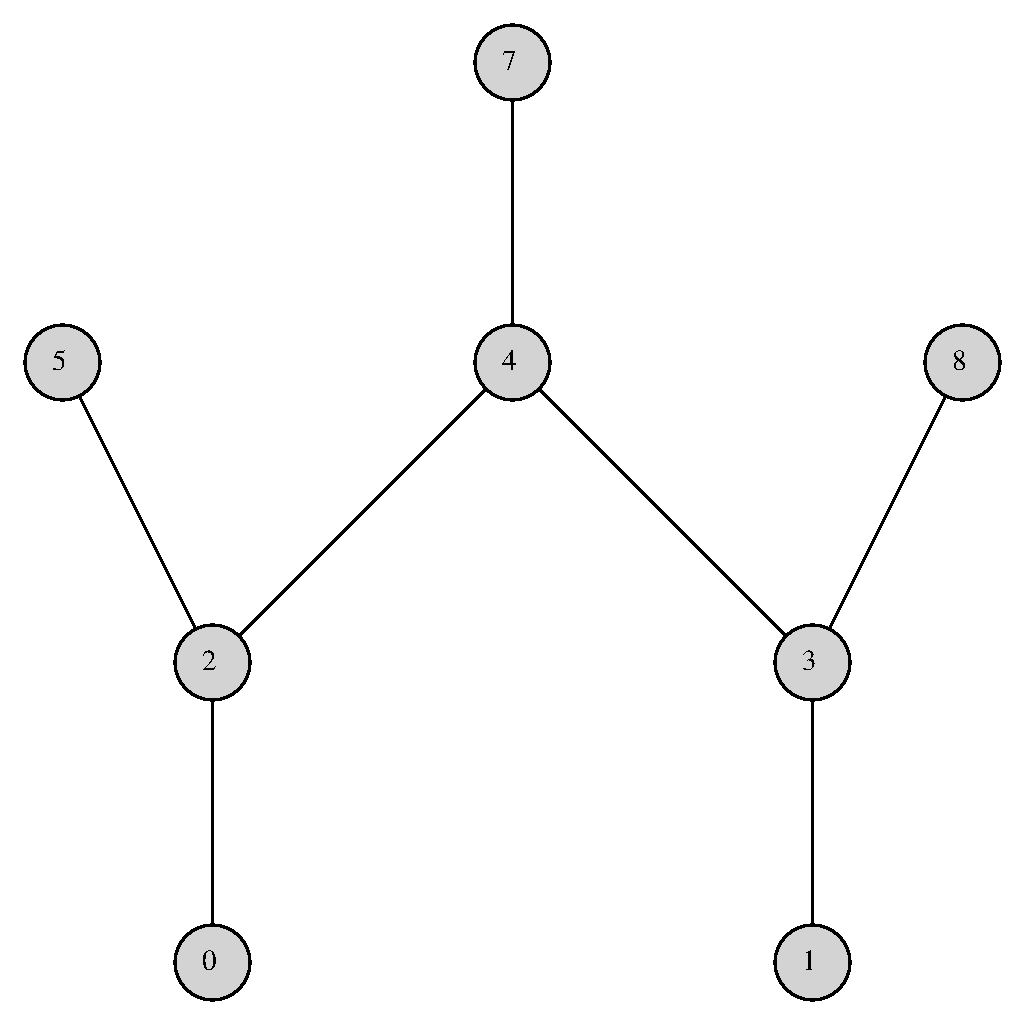
\includegraphics[scale=0.4]{./images/w3x3.eps}}}%
    \qquad
    \subfloat[Branch Decomposition.]{{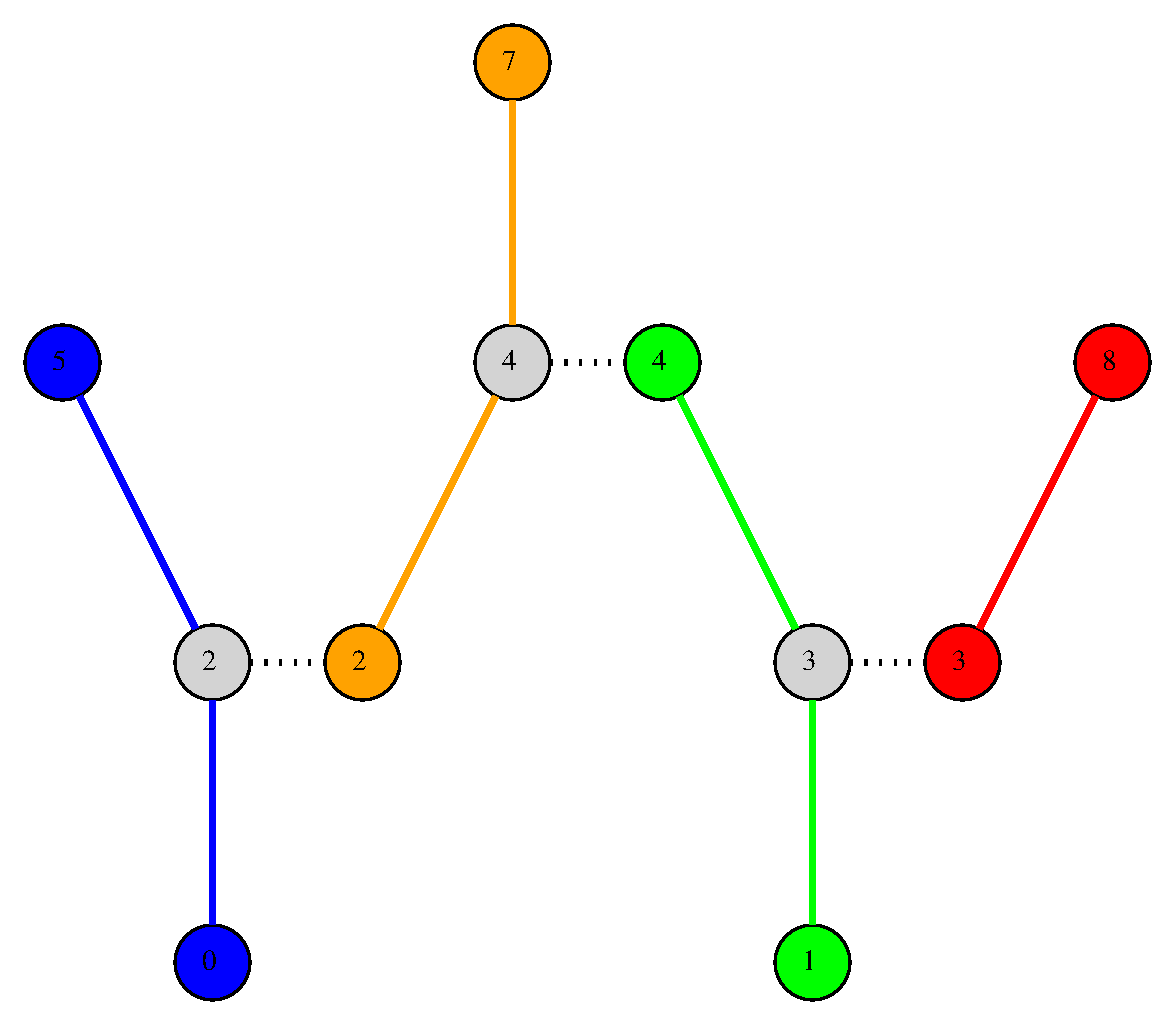
\includegraphics[scale=0.4 ]{./images/branch-decomposition-W3x3.eps}}}%
    \caption{Branch Decomposition of a Contour tree.}%
    \label{fig:example}%
\end{figure}

%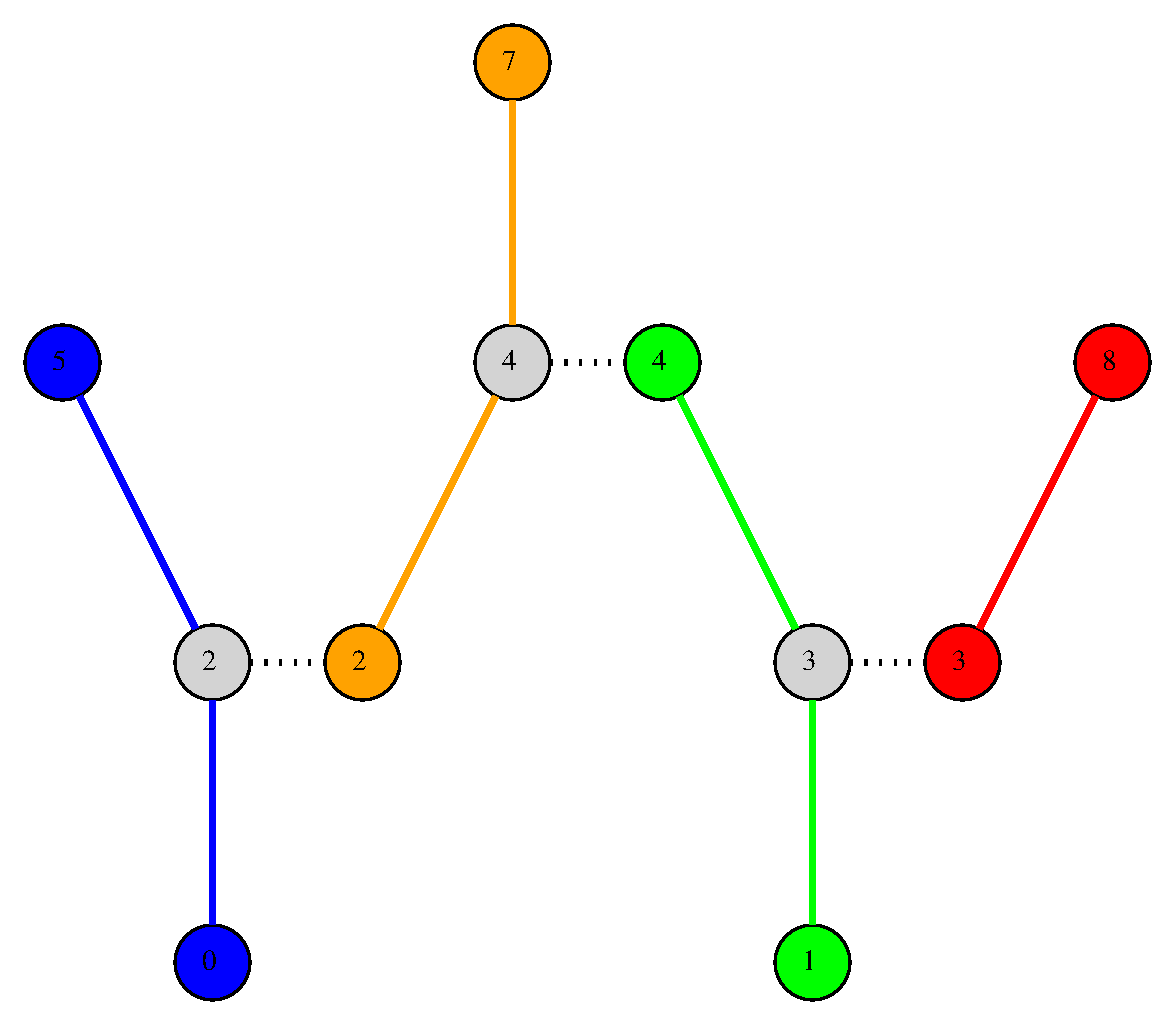
\includegraphics[center, scale=0.5 ]{./images/branch-decomposition-W3x3.eps}
%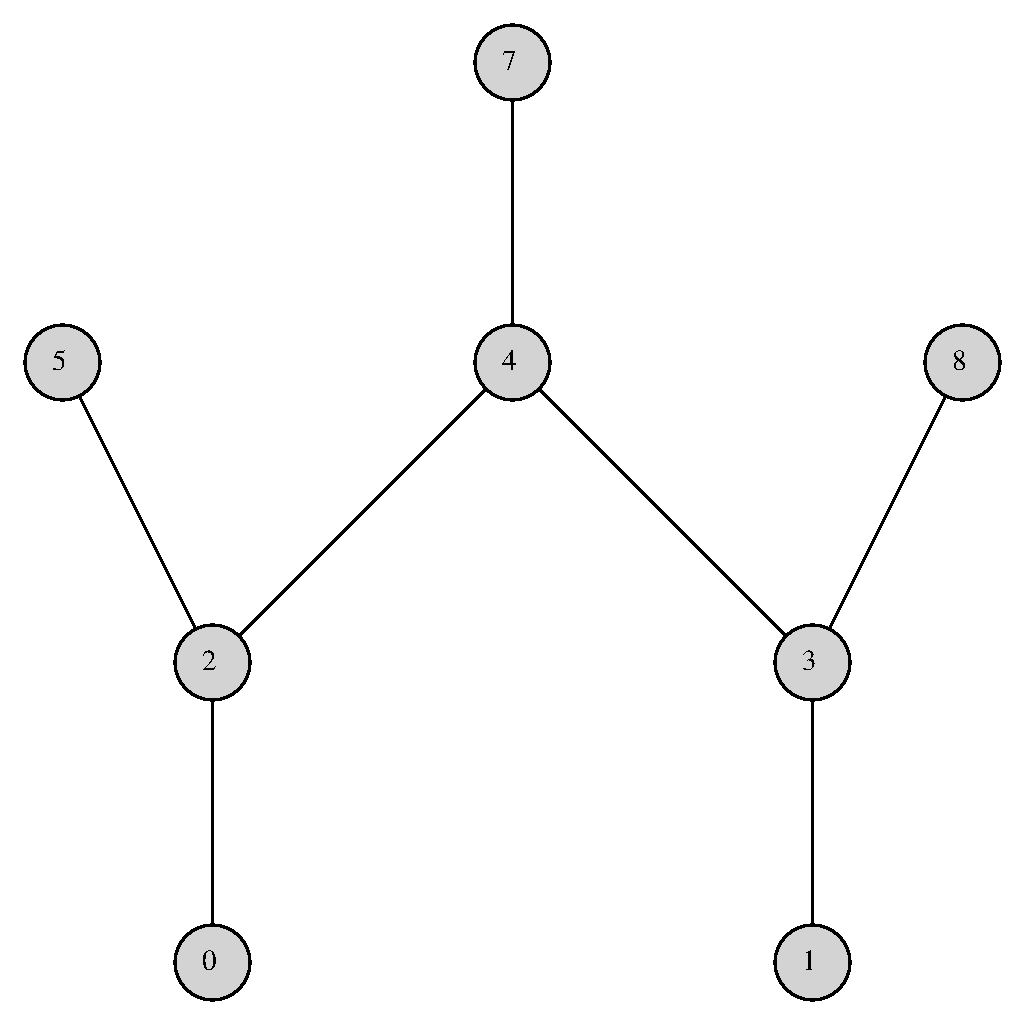
\includegraphics[center, scale=0.5]{./images/w3x3.eps}


% @TODO Todo talk about how this is used to remove noise and artifacts in data.

% @TODO Remove Stay Tuned
The paper \cite{ct-branch-decomp} cites that the persistence defined in that way is similar to persistence first defined in \cite{persistence-original}. In Chapter N of this dissertation we will demonstrate that this claim is either incorrect of misleading. Stay tuned folks.



%First we have to triangulate the mesh.

%Then the mesh is a height graph.

%And the contour tree is a height tree.

%Now define the join and split trees.

%Say they are equal for the mesh and the CT

%Compute the join/split tree of the mesh.

%Now combine them using the combination algorithm.

%There are many algorithms for computing the contour tree. But the Great Khan of all algorithms is the ONE. And then there's the parallel one!


\section{Additional Proofs}

\begin{lem} In a tree with no vertices of degree two at least half of the vertices are leaves. \end{lem}

\begin{proof}
    Let $T = (V, E)$ be a tree with no vertices of degree two and let $L \subseteq V$ be the set of all leaves. As all leaves have degree one we have that $L = \{u \in V: d(u) = 1\}$. Furthermore for any tree we know that $|E| = |V| - 1$. Let us now use the handshake lemma:

    $$ \sum_{u \in V}{d(u)} = 2|E| = 2(|V| - 1) = 2|V| - 2.$$

    We will not separe the sum on the leftmost hand side of the equation in two parts. One for the vertices vertices in $L$ and one for the vertices in $V\textbackslash L$.


    $$ \sum_{u \in L}{d(u)} + \sum_{u \in V\textbackslash L}{d(u)} = 2|V| - 2.$$

    All the vertices in $L$ are leaves. By definition the degree of a leaf is one. Therefore $\sum_{u \in L}{d(u)} = |L|$. This leads us to the following:

    $$  |L| + \sum_{u \in V\textbackslash L}{d(u)} = 2|V| - 2$$
    $$  |L|  = 2|V| - 2 - \sum_{u \in V\textbackslash L}{d(u)}.$$

    There are no vertices in $T$ of degree two and all vertices of degree one are in $L$. This means that all vertices in $V \textbackslash T$ have degree at least three. We can conclude that:
    $$\sum_{u \in V\textbackslash L}{d(u)} \ge \delta(T - L).|V\textbackslash L| = 3(|V| - |L|) $$

    Combining this with the previous equation we obtain that:

    $$  |L| \le 2|V| - 2 - 3(|V| - |L|)$$
    $$  |L| \le 2|V| - 2 - 3|V| + 3|L|$$
    $$  -2|L| \le -|V| - 2$$
    $$  |L| \ge \frac{|V|}{2} + 1$$

    Which is exactly what we set out to proove.


\end{proof}

\begin{lem} There are at least $k$ vertices for every vertex of degree $k$ in a tree. \end{lem}

\begin{proof}
    Let $T$ be a tree and $u \in V(T)$ be a vertex in it. As any tree can be rooted, let us root $T$ at $u$ and call the new directed tree $T_u$. Let $U = \{u_1, u_2, ..., u_k\}$ be the neighbours of $u$. For each $u_i \in U$ if $u_i$ is not a leaf let $u_i$ be one of it's children. Repeat this process until every $u_i$ is a leaf. This is possible because $T$ is finite. All of the $u_i$ are distinct, for otherwise there would be a cycle in $T$.
    
\end{proof}


% @TODO Redo this!
%For future reference we would also like to present a claim that is more general than this. Notice that we could have required that $T$ has no vertices of degree less than $n \in \{3, 4, 5, ...\}$. If we make the substitution accordingly we obain that:

    %$$\sum_{u \in V\textbackslash L}{d(u)} \ge n(|V| - |L|) $$

    %$$  |L| \ge \frac{n - 2}{n - 1}|V| + \frac{2}{n - 1}$$

    %As $n$ gets larger we have that $ \lim_{n \to \infty}\frac{2}{n - 1} = 0$ and by L'Hopital's rule:
    
    %$$\lim_{n \to \infty} \frac{n - 2}{n - 1} = \lim_{x \to \infty} \frac{(n - 2)'}{(n - 1)'} = 1$$

    %This means that for sufficiently large $n$ almost all of the vertices in a tree are leaves. Even for $n = 11$ we already have that at least $8/10$ of the vertices are leaves. This result will come in handy in one of the proofs in the second chapter.





%The contours of a contour tree are a subset of the join components. Therefore one join components corresponds to one or multiple contours. We will define the join tree as the graphs that represents join components and their evolution in time. As the join components can only grow bigger and never shrink there can be no cycles in graph and therefore the join tree is a tree.


%The first thing we shall do is redefine an analogue of the sublevel and superlevel sets of the height function in terms of subgraphs of the contour tree.

%The first and most important theoretical results comes from Morse Theory. It tells us that the critical values of a function which is a linear interpolation on a simplical mesh will be at the vertices of the simplical mesh. This key result implies that vertices in the contour tree correspond to vertices in the mesh. We will demonstrate how the current state of the art algorithms use this property to compute the Contour Tree just from the vertices of the mesh and their 1-dimensional connectivity.

%\begin{defn} Let $G$ be a height graph. The sublevel graph $\Gamma_i^-(G)$ of $G$ is the subgraph induced by the vertices of $G$ whose height is less than that of $v_i$.  \end{defn}

%The superlevel graph is defined analogously as $\Gamma_i^+(G)$ as the subgraph induces by the vertices of $G$ whose height is more than that of $v_i$. We will use the superlevel and sublevel graph the define the join and split trees respectively.

%\begin{defn}
    %Let $G$ be a Height Graph. The Join Tree $J_G$ of $G$ is a tree whose vertices are copies of those of $G$. If $V(G) = \{v_1, ..., v_n\}$ then $V(J_G) = \{p_1, ..., p_n\}$ where $h(p_i) = h(v_i), i \in 1, 2, ..., n$. Furthermore $p_ip_j \in E(J_G)$ for $i < j$ when:

%\end{defn}

%\begin{itemize}
    %\item $v_j$ is the vertex in some connected component of $\Gamma_i^+(G)$ with minimum height,
    %\item $v_i$ is adjacent to a vertex in that connected component.
%\end{itemize}

%We will make an analogous definition of the Split Tree which is $S_G$.

%\begin{defn}
    %Let $G$ be a Height Graph. The Split Tree $J_G$ of $G$ is a tree whose vertices are copies of those of $G$. If $V(G) = \{v_1, ..., v_n\}$ then $V(S_G) = \{s_1, ..., s_n\}$ where $h(s_i) = h(s_i), i \in 1, 2, ..., n$. Furthermore $s_is_j \in E(S_G)$ for $i < j$ when:

%\end{defn}

%\begin{itemize}
    %\item $v_j$ is the vertex in some connected component of $\Gamma_i^+(G)$ with maximum height,
    %\item $v_i$ is adjacent to a vertex in that connected component.
%\end{itemize}

%*SHOW EXAMPLES AND PRETTY PICTURES*

%One may notice that the if we only consider the vertices and edges of the input mesh we obtain a height graph of which we can compute the join and split tree. The main theoretical result established in \cite{carr-masters} is that the join and split trees of the input mesh and of the contour tree of that mesh are isomorphic. Therefore if we compute the join and split trees of the mesh we immediately obtain the join and split trees of the contour tree.

%An algorithm for compute the join and split trees of the mesh this is reported in \cite{carr-masters}. It operates by first performing an upwards sweep over all the vertices. It checks the connectivity of each vertex to determine which connected components it is connected to in $\Gamma_i^+$. It then add an edge in the join tree between the current vertex and the lowest vertex in that connected component. This sweep is followed by an analogous downwards sweep that computes the split tree of the mesh.

%As we alluded previously a contour tree has a unique pair of join and split trees. We will now present the algorithm for combining the join and split trees to produce the contour tree. The algorithm relies on a number of theoretical properties presented in \cite{carr-masters}. There are three key properties.

%\begin{itemize}
    %\item We can detect the leaves of the contour tree and their adjacent edge by looking at the join and split trees.
    %\item We can remove the leaves from the join and split tree. In doing this we obtain join and split trees for the contour tree excluding it's leaves.
    %\item We can continue this process of removing all the leaves inductively until we obtain the full contour tree.
%\end{itemize}

%*SHOW EXAMPLES AND PRETTY PICTURES*

%*SHOULD I GIVE ALL DETAIL EXPLICITELY?*

%\begin{lem} Given a height tree $T$ and it's join tree $J_T$ then $\delta_{T}^-(v) = \delta_{S_T}^-(v)$ and $\delta_{T}^+(v) = \delta_{J_T}^+(v)$.\end{lem}

%Therefore the following hold:

%\begin{lem} If $\delta_{J_T}^+(v) = 0$ and $\delta_{J_T}^-(v) = 1$ then $v$ is an \textbf{upper} leaf in $T$.\end{lem}
%\begin{lem} If $\delta_{J_T}^+(v) = 1$ and $\delta_{J_T}^-(v) = 0$ then $v$ is a \textbf{lower} leaf in $T$.\end{lem}

%Note that these vertices do not have to be leaves in either the join or split tree.

%On top of this we have that:

%We have seen that we can identify the leaves of a height tree by looking at the join and split trees. In fact we can do even better. We can identify the edge adjacent to those leaves.

%*DEFINE THE REDUCTION*

%*DEFINE HOW WE REDUCE BY MOVING ALL LEAVES TO THE CT FROM THE JOIN AND SPLIT*
